\begin{enumerate}[label=\thesubsection.\arabic*,ref=\thesubsection.\theenumi]
\item
Find the angle between the lines whose direction ratios are $a,b,c$ and $b-c,c-a,a-b$.
\\
\solution
    \begin{align}
\because \myvec{a&b&c}\myvec{b-c\\c-a\\a-b} = 0,
   \theta=\frac{\pi}{2}
    \end{align}

\item Name the type of quadrilateral formed, if any, by the following points,and give reasons for your answer
\begin{enumerate}
\item $A(-1,-2), B(1,0), (C-1,2), D(-3,0)$
\item $A(-3,5), B(-3,1), C(0,3), D(-1,-4)$
\item $A(4,5), B(7,6), C(4,3), D(1,2)$
\end{enumerate}
\solution
			See \tabref{tab:10/7/1/6/inner},
	\figref{fig:10/7/1/6/Fig1}, \figref{fig:10/7/1/6/Fig2}.
	and 
	\figref{fig:10/7/1/6/Fig3}. 
In b), forming the collinearity matrix
\begin{align}
\myvec{\vec{B}-\vec{A} & \vec{C}-\vec{B}} 
=
		\myvec{6&-3\\-4&2} \xleftrightarrow{R_{2}\rightarrow R_{2}+\frac{2}{3}R_{1}}= \myvec{6&-3\\0&0}
\end{align}
which is a rank 1 matrix.  Hence, $\vec{A}, \vec{B}, \vec{C}$  are collinear.
\begin{figure}[H]
	\begin{center} 
	    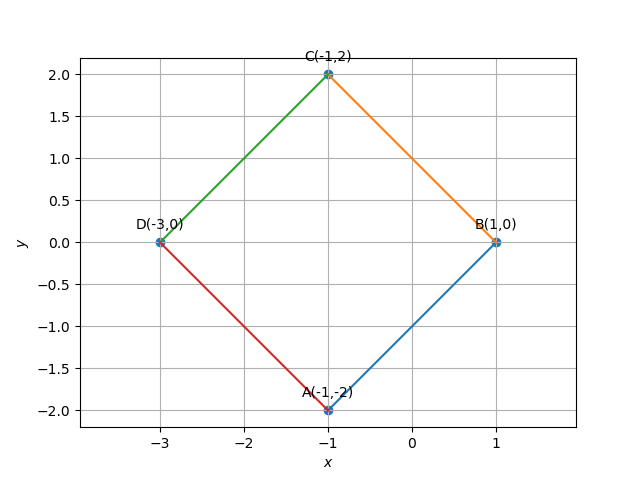
\includegraphics[width=0.75\columnwidth]{chapters/10/7/1/6/figs/quad1}
	\end{center}
\caption{}
\label{fig:10/7/1/6/Fig1}
\end{figure}
%
\begin{figure}[H]
	\begin{center} 
	    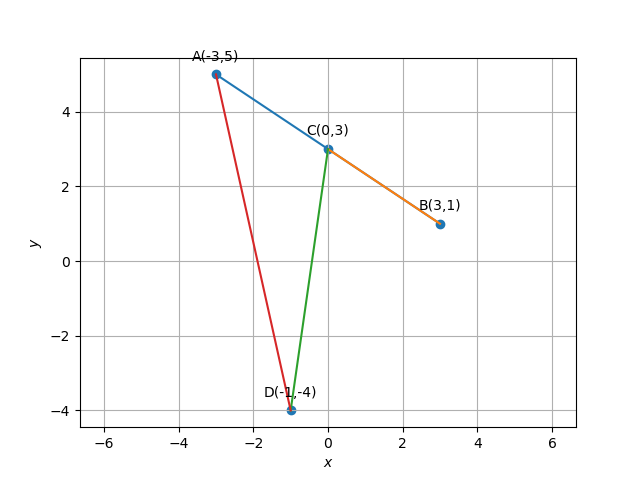
\includegraphics[width=0.75\columnwidth]{chapters/10/7/1/6/figs/quad2}
	\end{center}
\caption{}
\label{fig:10/7/1/6/Fig2}
\end{figure}
%	
\begin{figure}[H]
	\begin{center} 
	    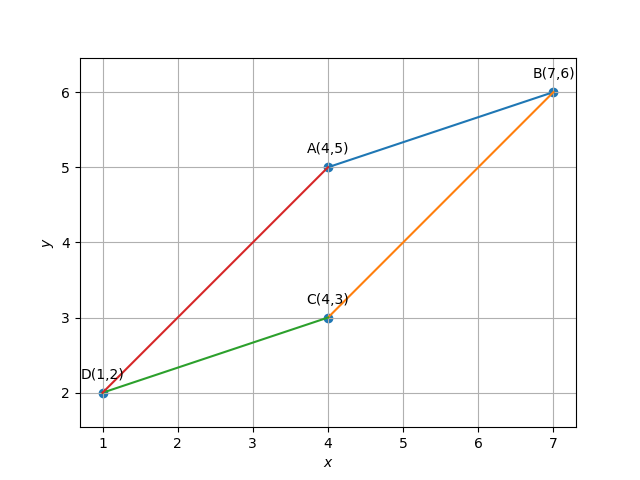
\includegraphics[width=0.75\columnwidth]{chapters/10/7/1/6/figs/quad3}
	\end{center}
\caption{}
\label{fig:10/7/1/6/Fig3}
\end{figure}
%
\begin{table}[H]
    \centering
%    \begin{tabular}{|c|c|c|c|c|}
	    \begin{tabularx}{\columnwidth}{|c|X|X|X|c|}
        \hline
		    &{\scriptsize $\vec{B}-\vec{A} = \vec{C}-\vec{D}$?} & {\tiny $(\vec{B}-\vec{A})^\top (\vec{C}-\vec{B}) =  0$?} & {\tiny $(\vec{C}-\vec{A})^\top (\vec{D}-\vec{B}) = 0$}& \textbf{Geometry}\\
        \hline
	    a)& Yes & Yes & Yes& Square \\
        \hline
	    b)& No & -&- & Triangle\\
        \hline
	    c)&Yes & No & No & Parallelogram\\
        \hline
	\end{tabularx}
%    \end{tabular}
	\caption{}
	\label{tab:10/7/1/6/inner}
\end{table}

\item Find the projection of the vector $\hat{i}+3\hat{j}+7\hat{k}$ on the vector $7\hat{i}-\hat{j}+8\hat{k}$.
	\\
	\solution
				Let 
\begin{align}
 \vec{A} =\myvec{1\\3\\7}, \vec{B} =\myvec{7\\-1\\8}
\end{align}
The projection of $\vec{A}$ on $\vec{B}$ is defined as
the foot of the perpendicular from 
$\vec{A}$ to $\vec{B}$ and obtained in 
	\eqref{eq:12/10/3/4/proj}.
Substituting numerical values,
\begin{align}
	\vec{C}
		=\frac{10}{19}\myvec{7\\-1\\8}
 \end{align}

\item Find the projection of the vector $\hat{i}-\hat{j}$ on the vector $\hat{i}+\hat{j}$.
	\\
\solution
		The given points are
\begin{align}
 \vec{A}=\myvec{1\\ -1},
 \vec{B}=\myvec{1\\ 1}
\end{align}
Since
\begin{align}
	\vec{A}^\top \vec{B} =0,
\end{align}
	from \eqref{eq:12/10/3/4/proj},
the projection vector is the origin.
		See \figref{fig:12/10/3/3fig}.
\begin{figure}[H]
	\centering
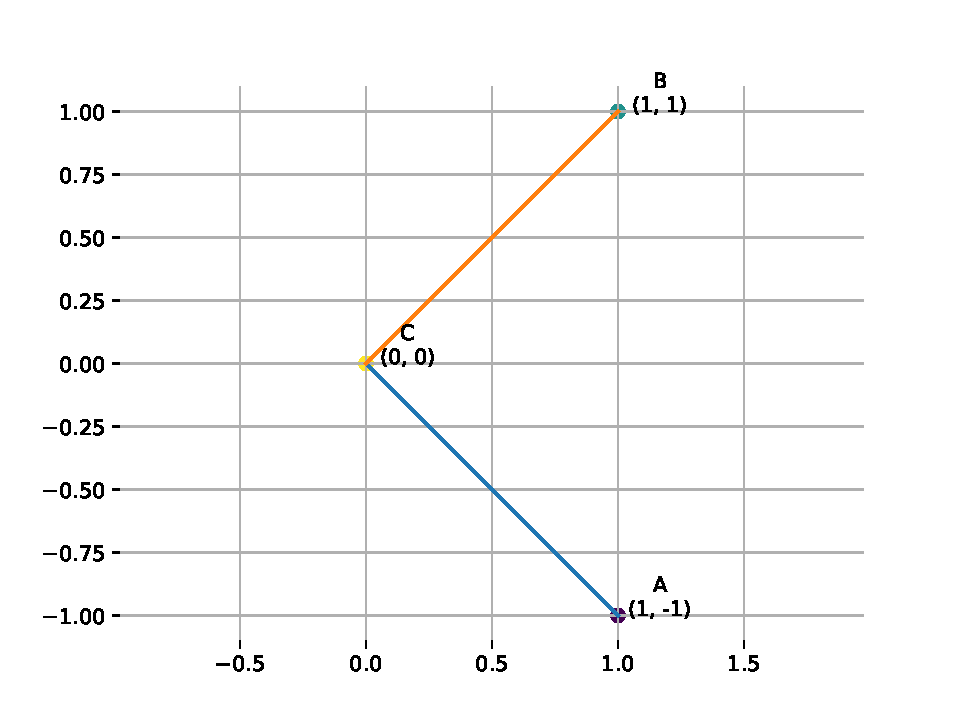
\includegraphics[width=0.75\columnwidth]{chapters/12/10/3/3/figs/fig.pdf}
\caption{}
		\label{fig:12/10/3/3fig}
\end{figure}

\item Show that each of the given three vectors is a unit vector: 
 $\frac{1}{7}(2\hat{i}+3\hat{j}+6\hat{k}),\frac{1}{7}(3\hat{i}-6\hat{j}+2\hat{k}),\frac{1}{7}(6\hat{i}+2\hat{j}-3\hat{k}$).
Also,show that they are mutually perpendicular to each other.
	\\
	\solution
		\begin{align}
\vec{A} = 	\myvec{
	\frac{2}{7} & \frac{3}{7} & \frac{6}{7} \\[1ex]
    \frac{3}{7} & -\frac{6}{7} & \frac{2}{7} \\[1ex]
    \frac{6}{7} & \frac{2}{7} & -\frac{3}{7}
}
\end{align}
is an orthogonal matrix satisfying
\eqref{eq:12/10/3/5/inner},
which verifies the given conditions.

\item If $\overrightarrow {a}=2\hat{i}+2\hat{j}3\hat{k},\overrightarrow {b}=\hat{-i}+2\hat{j}+\hat{k}$ and $\overrightarrow {c}=3\hat{i}+\hat{j}$ are such that $\overrightarrow {a}+\lambda\overrightarrow {b}$ is perpendicular to $\overrightarrow {c}$,then find the value of $\lambda$.
	\\
		\solution
\begin{align}
\because	(\vec{a}+\lambda \vec{b})^{\top} \vec{c} = 0,
	\\
	\lambda=-\frac{\vec{a}^{\top}\vec{c}}{\vec{b}^{\top}\vec{c}}
	=8,
\end{align}
upon substituting numerical values.



\item Show that $\abs {\overrightarrow {a}}\overrightarrow {b}+\abs{\overrightarrow {b}}\overrightarrow {a}$ is perpendicular to $\abs{\overrightarrow {a}} \overrightarrow {b}-\abs{\overrightarrow {b}} \overrightarrow {a}$, for any two nonzero vectors $\overrightarrow {a}$ and $\overrightarrow {b}$.
	\\
	\solution
		\begin{align}
\norm{\vec{a}}\vec{b}+\norm{\vec{b}}\vec{a}
=
	\norm{\vec{a}}\norm{\vec{b}}\brak{\frac{\vec{b}}{\norm{\vec{b}}}+\frac{\vec{a}}{\norm{\vec{a}}}}
	\\
\norm{\vec{a}}\vec{b}-\norm{\vec{b}}\vec{a}
=
	\norm{\vec{a}}\norm{\vec{b}}\brak{\frac{\vec{b}}{\norm{\vec{b}}}-\frac{\vec{a}}{\norm{\vec{a}}}}
	\\
	\implies 
	\brak{\norm{\vec{a}}\vec{b}+\norm{\vec{b}}\vec{a}}^{\top} \brak{\norm{\vec{a}}\vec{b}-\norm{\vec{b}}\vec{a}} = 0
\end{align}
	from \eqref{eq:12/10/3/11/unit}.

\item If $\overrightarrow {a},\overrightarrow {b},\overrightarrow {c}$ are unit vectors such that $\overrightarrow {a}+\overrightarrow {b}+\overrightarrow {c}=\overrightarrow {0}$, find the value of $\overrightarrow {a}.\overrightarrow {b}+\overrightarrow {b}.\overrightarrow {c}+\overrightarrow {c}.\overrightarrow {a}$.
	\\
	\solution
		\begin{align}
	\norm{{\vec{a}}+{\vec{b}}+{\vec{c}}}^2=0
	\nonumber \\
	\implies{\norm{\vec{a}}}^2+{\norm{\vec{b}}}^2+{\norm{\vec{c}}}^2+2({{\vec{a}^\top}{\vec{b}}+{\vec{b}^\top}{\vec{c}}+{\vec{c}^\top}{\vec{a}}})=0
	\nonumber \\
	\implies3+2({{\vec{a}^\top}{\vec{b}}+{\vec{b}^\top}{\vec{c}}+{\vec{c}^\top}{\vec{a}}})=0\nonumber \\
	\implies{\vec{a}^\top}{\vec{b}}+{\vec{b}^\top}{\vec{c}}+{\vec{c}^\top}\vec{a}=-\frac{3}{2}
\end{align}

\item If either vector $\overrightarrow {a}=0$ or $\overrightarrow {b}=0$, then $\overrightarrow {a}.\overrightarrow {b}$=0. But the converse need not be true. Justify your answer with an example.
	\\
	\solution
		\begin{align}
	\vec{a}=\myvec{1\\1},\,
\vec{b}=\myvec{1\\-1}\\
\implies \vec{a} ^\top \vec{b} =  0 
\end{align}



\item Show that the vectors $2\hat{i}-\hat{j}+\hat{k},\hat{i}-3\hat{j}-5\hat{k}$ and  $3\hat{i}-4\hat{j}-4\hat{k}$ from the vertices of a right angled triangle.
	\\
	\solution
		\begin{align}
\vec{A} = \myvec{2\\-1\\1}, \, \vec{B} = \myvec{1\\-3\\-5}, \, \vec{C}=\myvec{3\\-4\\-4},
\\
\implies \vec{B}-\vec{C} = \myvec{-2\\1\\-1} ,\, 
\vec{C}-\vec{A} = \myvec{1\\-3\\-5} ,\, 
\\
	\text{or, }
\brak{\vec{B}-\vec{C}}^{\top}\brak{\vec{C}-\vec{A}} = 0
\end{align}

\item Show that the points A, B and C with position vectors, $3\hat{i}-4\hat{j}-4\hat{k}, 2\hat{i}-\hat{j}+\hat{k}$ and $\hat{i}-3\hat{j}-5\hat{k}$, respectively, form the vertices of a right angled
triangle.
\\
\solution
		    \begin{align}
         \vec{B} - \vec{A} = \myvec{-1\\3\\5},\, 
         \vec{C} - \vec{B} = \myvec{-1\\-2\\-6},\,
         \vec{C} - \vec{A} = \myvec{-2\\1\\-1},
        \label{eq:chapters/12/10/2/17/dir-vec}
	\\
	    \implies 
	    \brak{\vec{B} - \vec{A}}^\top
	    \brak{\vec{C} - \vec{A}} = 0
    \end{align}
Hence, $\triangle ABC$ is right angled at $\vec{A}$. 

\item Let $\vec{a}=\hat{i}+4\hat{j}+2\hat{k}, \vec{b}=3\hat{i}-2\hat{j}+7\hat{k}$ and $\vec{c}=2\hat{i}-\hat{j}+4\hat{k}$. Find a vector $\vec{d}$ which is perpendicular to both $\vec{a}$ and $\vec{b}$, and $\vec{c}\cdot \vec{d}$=15.\\
	\solution
		From the given information, 
\begin{align}
\vec{a}^{\top}\vec{d} &= 0\\
\vec{b}^{\top}\vec{d} &= 0\\
\vec{c}^{\top}\vec{d} &= 15
\end{align}
yielding
\begin{align}
\myvec{\vec{a}^{\top} \\\vec{b}^{\top}\\\vec{c}^{\top}}\vec{d} &= \myvec{0\\0\\15}\\
\implies \myvec{1&4&2 \\3&-2&7 \\2&-1&4}\vec{d} &= \myvec{0\\0\\15}
\label{eq:chapters/12/10/5/12/1}
\end{align}
%
Forming the augmented matrix, 
\begin{align}
	\myvec{1&4&2&\vrule&0\\ 3&-2&7&\vrule&0 \\ 2&-1&4&\vrule&15} 
	\xleftrightarrow[R_3\leftarrow R_3-2R_1]{R_2\leftarrow R_2-3R_1}
	\myvec{1&4&2&\vrule&0\\ 0&-14&1&\vrule&0 \\ 0&-9&0&\vrule&15}
\nonumber	\\
	\xleftrightarrow[]{R_3\leftarrow R_3-\frac{9}{14}R_2}
	\myvec{1&4&2&\vrule&0\\ 0&-14&1&\vrule&0 \\ 0&0&-\frac{9}{14}&\vrule&15}
	\label{eq:chapters/12/10/5/12/2}
\end{align}
yielding
%
\begin{align}
	\vec{d} &= \myvec{\frac{160}{3}\\[1ex]-\frac{5}{3}\\[1ex]-\frac{70}{3}}
\end{align}
upon back substitution.


\item Prove that $(\vec{a}+\vec{b})\cdot(\vec{a}+\vec{b})=|{\vec{a}}|^2+|{\vec{b}}|^2$, if and only if $\vec{a}, \vec{b}$ are perpendicular, given $\vec{a}\neq\vec{0}, \vec{b}\neq\vec{0}$.\\
	\solution
			\begin{align}
\because 		\brak{\vec{a}+\vec{b}}^{\top}\brak{\vec{a}+\vec{b}} 
		= \norm{\vec{a}}^2+\norm{\vec{b}}^2,
		\\
		 \norm{\vec{a}}^2+\norm{\vec{b}}^2+2\vec{a}^{\top}\vec{b}
		= \norm{\vec{a}}^2+\norm{\vec{b}}^2
		\\
		\implies 
		\vec{a}^{\top}\vec{b} = 0 
	\end{align}


\item $ABCD$ is a rectangle formed by the points $\vec{A}(–1, –1), \vec{B}(– 1, 4), \vec{C}(5, 4)$  and  $\vec{D}(5, – 1)$. $\vec{P}, \vec{Q}, \vec{R}$ and $\vec{S}$ are the mid-points of $AB, BC, CD$ and $DA$ respectively. Is the quadrilateral $PQRS$ a square? a rectangle? or a rhombus? Justify your answer.
	\\
	\solution 
See Fig. \ref{fig:10/7/4/8Fig3}. From 
  \eqref{eq:10/7/4/8det2f}, $PQRS$ is a parallelogram.
\begin{align}
  %\label{eq:10/7/4/8det2f}
  \vec{P}  = 
 \frac{3}{2},\, 
 \vec{Q}  = \myvec{
 2 \\
 4 \\
 } ,\,
 \vec{R}  = \myvec{
 5 \\
 \frac{3}{2}
 }   
  ,\,
 \vec{S}  = \myvec{
 2\\
 -1 \\
 }   
 \\
	\implies 
 \brak{\vec{Q}-\vec{P}}^\top\brak{\vec{R}-\vec{Q}}  \neq 0
 \\
 \brak{\vec{R}-\vec{P}}^\top\brak{\vec{S}-\vec{Q}}  = 0
\end{align}
Therefore $PQRS$ is a rhombus.
\begin{figure}[!h]
	\begin{center}
		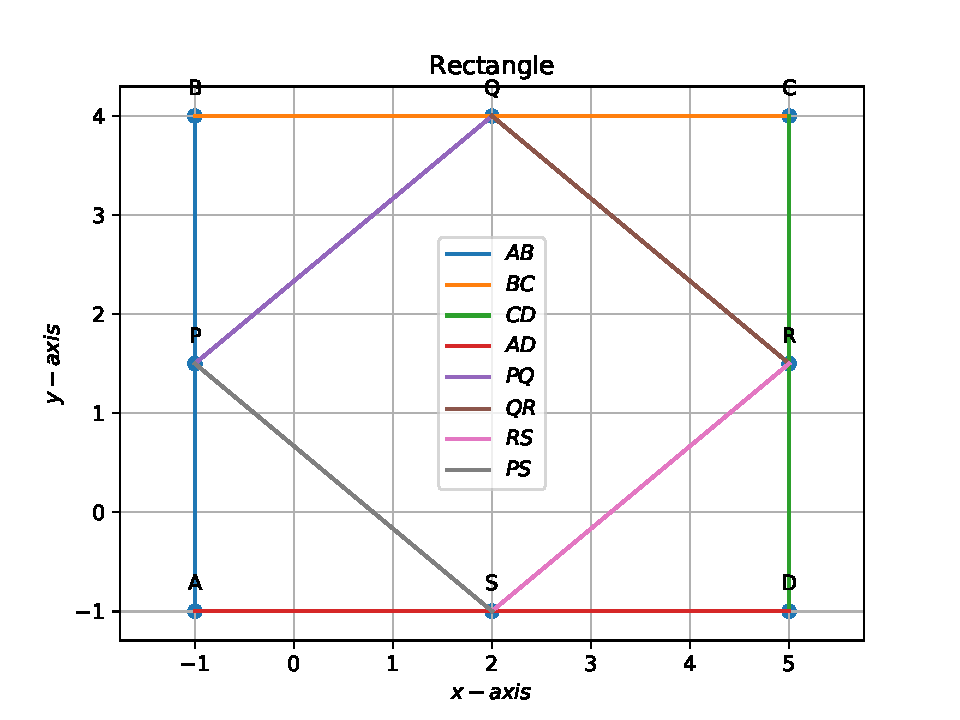
\includegraphics[width=\columnwidth]{chapters/10/7/4/8/figs/problem1.pdf}
	\end{center}
\caption{}
\label{fig:10/7/4/8Fig3}
\end{figure}


\item Without using the Baudhayana theorem, show that the points $A(4,4), B(3,5)$ and $C(-1,-1)$ are the vertices of a right angled triangle.
\label{chapters/11/10/1/6}
		See \figref{fig:11/10/1/6}.
\begin{align}
	\vec{C}-\vec{A}=\myvec{
-5 \\
	-5},\,
	\vec{A}-\vec{B}&=\myvec{
1 \\
-1 
}
\\
	\implies \brak{\vec{C}-\vec{A}}^{\top}
	\brak{\vec{A}-\vec{B}}&=0
\end{align}
Thus, $AB \perp AC$.
	\begin{figure}[H]
		\centering
 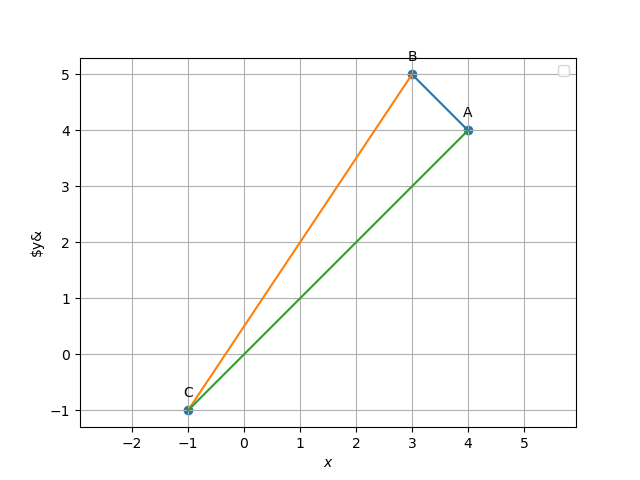
\includegraphics[width=0.75\columnwidth]{chapters/11/10/1/6/figs/triangle.png}
		\caption{}
		\label{fig:11/10/1/6}
  	\end{figure}

\item The line through the points $(h, 3)$ and $(4, 1)$ intersects the line $7x- 9y- 19= 0$ at a right angle. Find the value of $h$.
\label{chapters/11/10/3/10}
\\
\solution
The direction vectors of the given lines are 
\begin{align}
\myvec{4-h\\ -2}
,\,
\myvec{9\\ 7}
\\
\implies 
\myvec{9& 7}\myvec{4-h\\ -2}=0\\
\implies h=\frac{22}{9}
\end{align}
See  
		\figref{fig:chapters/11/10/3/10/Figure}.
\begin{figure}[h]
\centering
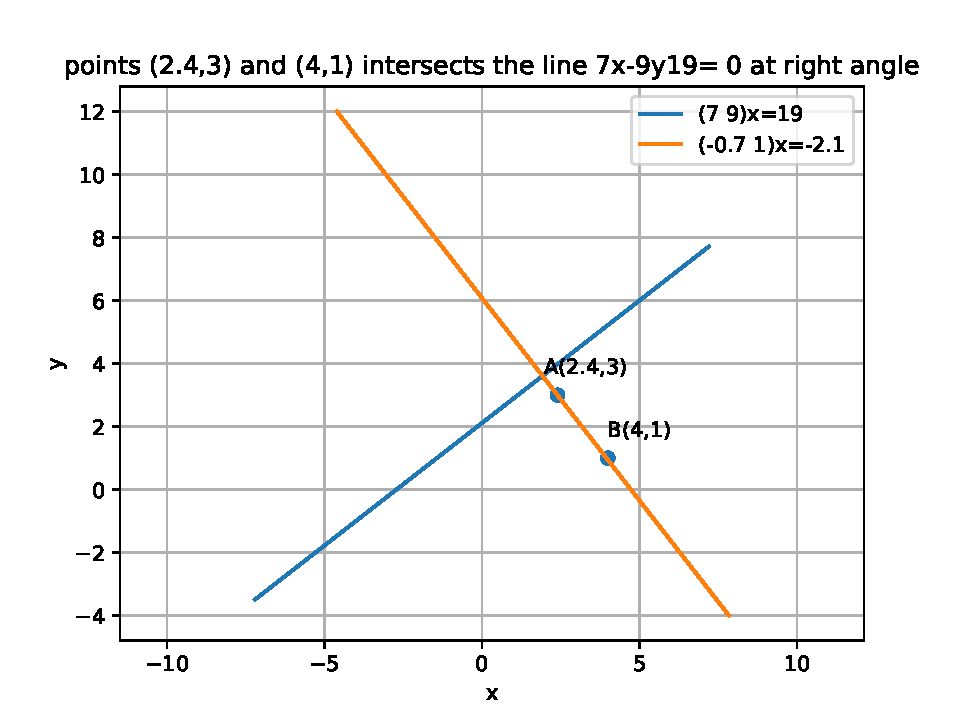
\includegraphics[width=\columnwidth]{chapters/11/10/3/10/figs/fig.pdf}
\caption{}
		\label{fig:chapters/11/10/3/10/Figure}
\end{figure}

\item In the following cases, determine whether the given planes are parallel or perpendicular, and in case they are neither, find the angles between them.
\begin{enumerate}
\item $7x + 5y + 6z + 30 = 0$ and $3x – y – 10z + 4 = 0$
\item $2x + y + 3z – 2 = 0$ and $x – 2y + 5 = 0$
\item $2x – 2y + 4z + 5 = 0$ and $3x – 3y + 6z – 1 = 0$
\item $2x – y + 3z – 1 = 0$ and $2x – y + 3z + 3 = 0$
\item $4x + 8y + z – 8 = 0$ and $y + z – 4 = 0$
\end{enumerate}
    \solution
		    See \tabref{tab:12/11/3/13}.
\begin{table}[htbp]
    \centering
    \caption{}
    \label{tab:12/11/3/13}
    \begin{tabular}{|c|c|c|c|c|c|}
        \hline
        $\vec{n}_1$ & $\vec{n}_1$ & $\vec{n}_1^{\top}\vec{n}_2$ & $\norm{\vec{n}_1}$ & $\norm{\vec{n}_2}$ & Angle\\
        \hline
        $\myvec{7\\5\\6}$ & $\myvec{3\\-1\\-10}$ & $-44$ & $\sqrt{110}$ & $\sqrt{110}$ & $\cos^{-1}-\frac{2}{5}$ \\
        \hline
        $\myvec{2\\1\\3}$ & $\myvec{1\\-2\\0}$ & $0$ & & & perpendicular \\
        \hline
        $\myvec{2\\-2\\4}$ & $\myvec{3\\-3\\6}$ & $36$ & $\sqrt{24}$ & $\sqrt{54}$ & parallel \\
        \hline
        $\myvec{2\\-1\\3}$ & $\myvec{2\\-1\\3}$ & $14$ & $\sqrt{14}$ & $\sqrt{14}$ & parallel \\
        \hline
        $\myvec{4\\8\\1}$ & $\myvec{0\\1\\1}$ & $9$ & $9$ & $\sqrt{2}$ & $45\degree$ \\
        \hline
    \end{tabular}
\end{table}

\iffalse
\begin{table}[htbp]
    \centering
    \caption{}
    \label{}
    \begin{tabular}{|c|c|c|c|c|c|}
        \hline
	    $\vec{n}_1$ & $\vec{n}_1$ &  $\vec{n}_1^{\top}\vec{n}_2$& $\norm{\vec{n}_1}$ &$\norm{\vec{n}_2}$  &  Angle\\
        \hline
	    \myvec{7\\5\\6} & \myvec{3\\-1\\-10} & -44 & \sqrt{110} &\sqrt{110}  & \cos^{-1}-\frac{2}{5} \\
        \hline
\myvec{2\\1\\3}  & \myvec{1\\-2\\0}& 0 &  &  & perpendicular\\
        \hline
 \myvec{2\\-2\\4} & \myvec{3\\-3\\6} & 36  & \sqrt{24} & \sqrt{54} &  parallel \\
        \hline
 \myvec{2\\-1\\3} & \myvec{2\\-1\\3} & 14 & \sqrt{14} & \sqrt{14} & parallel \\
        \hline
 \myvec{4\\8\\1} & \myvec{0\\1\\1} & 9 & 9 & \sqrt{2} &  45\degree  \\
        \hline
    \end{tabular}
\end{table}
\fi

		\item 
 Show that the line joining the origin to the point $P(2, 1, 1)$ is perpendicular to the
line determined by the points $A(3, 5, – 1), B(4, 3, – 1)$.
\\
    \solution
				\begin{align}
			\brak{\vec{A}-\vec{B}}^\top\vec{P}=
			\myvec{-1&2&0}\myvec{2\\1\\1}=0 \qed
		\end{align}

	\item  If $l_1, m_1,n_1 \text{ and } l_2,m_2,n_2$ are the direction cosines of two mutually perpendicular lines, show that the direction cosines of the line perpendicular to both these are  $m_1n_2-m_2n_1,n_1l_2-n_2l_1,l_1m_2-l_2m_1$.
\\
    \solution
		\begin{align}
\vec{P} 
	=\myvec{
l_1&l_2&m_1n_2-m_2n_1\\
        m_1&m_2&n_1l_2-n_2l_1\\
        n_1&n_2&l_1m_2-l_2m_1
}
	\end{align}
	satisfies 
\eqref{eq:12/10/3/5/inner}.
	Hence, the three vectors are mutually perpendicular.

	\item If the lines $\frac{x-1}{-3} = \frac{y-2}{2k} = \frac{z-3}{2}$ and  $\frac{x-1}{3k} = \frac{y-1}{1} = \frac{z-6}{-5}$ are perpendicular, find the value of $k$.\\
    \solution
		From the given information,
\begin{align}
\vec{m}_1 = \myvec{-3\\ 2k\\ 2},\,  \vec{m}_2 =\myvec{3k\\ 1\\ -5} 
\\
	\implies \myvec{-3& 2k& 2}^{\top} \myvec{3k\\ 1\\ -5} =0
	\\
	\implies k = -\frac{10}{7}
\end{align}
See 
     \figref{fig:chapters/12/11/4/6/1}
\begin{figure}[h!]
  \centering
   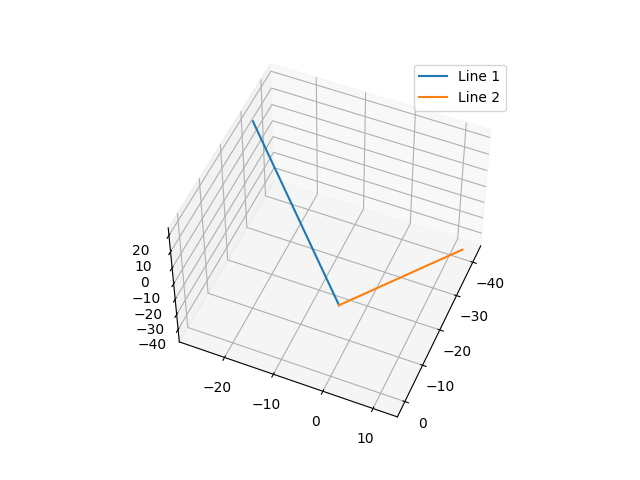
\includegraphics[width=\columnwidth]{chapters/12/11/4/6/figs/line_1.png}
    \caption{lines represented for the given points and direction vector with k=$\frac{-10}{7}$}
     \label{fig:chapters/12/11/4/6/1}
     \end{figure}  



\item If $\vec{a},\vec{b},\vec{c}$ are mutually perpendicular vectors of equal magnitudes, show that the vector $\vec{c}\cdot\vec{d}$=15 is equally inclined to $\vec{a},\vec{b}$ and $\vec{c}$.
    \item If $ \vec{A},\vec{B},\vec{C} $ are mutually perpendicular vectors of equal magnitudes,show that the  $ \vec{A}+\vec{B}+\vec{C} $ is equally inclined to $ \vec{A},\vec{B}  \text{ and }  \vec{C} $.
\item Check whether $(5,-2), (6,4)$ and $(7,-2)$ are the vertices of an isosceles triangle.
\item The perpendicular bisector of the line segment joining the points $\vec{A} (1, 5) \text{ and }
\vec{B} (4, 6)$ cuts the y-axis at
\begin{enumerate}
	\item$(0, 13)$ 
	\item $(0, –13)$
	\item$(0, 12) $
	\item$(13, 0)$
\end{enumerate}
\item The point which lies on the perpendicular bisector of the line segment joining the
	points $\vec{A} (–2, –5)\text { and } \vec{B} (2, 5) $ is
\begin{enumerate}
\item  	$(0, 0)$
\item  $(0, 2)$ 
\item  $(2, 0)$ 
\item  $(–2, 0)$
\end{enumerate}
\item The points $ (–4, 0), (4, 0), (0, 3) $ are the vertices of
	\begin{enumerate}
\item right triangle 
\item isosceles triangle
\item  equilateral triangle
\item  scalene triangle 
\end{enumerate}
\item The point $\vec{A}(2,7)$ lies on the perpendicular bisector of line segment joining the points $\vec{P}(6,5)\text{ and } \vec{Q}(0,-4)$.
\item The points $\vec{A}(-1,-2), \vec{B}(4,3), \vec{C}(2,5) \text{ and } \vec{D}(-3,0)$ in that order form a rectangle.
\item Name the type of triangle formed by the points $\vec{A}(-5,6),\vec{B}(-4,-2),\text{ and }\vec{C}(7,5)$.
\item What type of a quadrilateral do the points $\vec{A}(2,-2),\vec{B}(7,3),\vec{C}(11,-1),\text{ and }\vec{D}(6,-6)$ taken in that order, form?
\item Find the coordinates of the point $\vec{Q}$ on the $x$-axis which lies on the perpendicular bisector of the line segment joining the points $\vec{A}(-5,-2) \text{ and } \vec{B}(4,-2)$. Name the type of triangle formed by points $\vec{Q},\vec{A}\text{ and }\vec{B}$.
\item The points $\vec{A}(2,9),\vec{B}(a,5) \text{ and }\vec{C}(5,5)$ are the vertices of a triangle $\vec{ABC}$ right angled at $\vec{B}$. Find the values of a and hence the area of $\triangle \vec{ABC}$.
\item Find a vector of magnitude 6, which is perpendicular to both the vectors $2\hat{i}-\hat{j}$+$2\hat{k}\text{ and }4\hat{i}-\hat{j}+3\hat{k}$.
\item If A,B,C,D  are the points with position vectors $\hat{i}+\hat{j}-\hat{k}$, $2\hat{i}-\hat{j}+3\hat{k}$, $2\hat{i}-3\hat{k}$, $3\hat{i}$-$2\hat{j}$+$\hat{k}$, respectively, find the projection of $\overline{AB}$ $\text{ along }$ $\overline{CD}$.
\item Find the value of $\lambda$ such that the vectors $\vec{a}=2\hat{i}+\lambda\hat{j}+\hat{k}$ $\text{and}$ $\vec{b}=\hat{i}+2\hat{j}+3\hat{k}$ are orthogonal.
	\begin{enumerate}
\item 0
\item 1 
\item $\frac{3}{2}$
\item $-\frac{5}{2}$
	\end{enumerate}
\item Projection vector of $\vec{a}$ on $\vec{b}$ is
	\begin{enumerate}
\item $\left(\dfrac{\vec{a}\cdot\vec{b}}{\abs{\vec{b}}^2}\right)$
\item $\frac{\vec{a}\cdot\vec{b}}{\abs{\vec{b}}}$
\item $\frac{\vec{a}\cdot\vec{b}}{\abs{\vec{a}}}$
\item $\left(\dfrac{\vec{a}\cdot\vec{b}}{\abs{\vec{a}}^2}\right)$
\end{enumerate}
\item The vectors $\lambda\hat{i}+\lambda\hat{j}+2\hat{k}$, $\hat{i}+\lambda\hat{j}-\hat{k}$ $\text{ and }$ $2\hat{i}-\hat{j}+\lambda\hat{k}$ are coplanar if
	\begin{enumerate}
\item	$\lambda=-2$
\item $\lambda=0$
\item $\lambda=1$
\item	$\lambda=-1$
\end{enumerate}
\item The number of vectors of unit length perpendicular to the vectors $\vec{a}=2\hat{i}+\hat{j}+2\hat{k}$ $\text{ and }$ $\vec{b}=\hat{j}+\hat{k}$ is
	\begin{enumerate}
\item one
\item  two
\item three
\item infinite
\end{enumerate}
\item If $\vec{r}\cdot\vec{a}=0, \vec{r}\cdot\vec{b}=0$ and $\vec{r}\cdot\vec{c}=0$ for some non-zero vector $\vec{r}$, then the value of $\vec{a}\cdot(\vec{b}\times\vec{c})$ is \rule{1cm}{0.15mm}.
\item If $\abs{\vec{a}+\vec{b}}$ = $\abs{\vec{a}-\vec{b}}$, then the vectors $\vec{a}$ $\text {and}$ $\vec{b}$ are orthogonal.
\item Prove that the lines $x=py+q , z=ry+s \text{ and } x=p^{\prime}y+q^{\prime}, z=r^{\prime}y+s^{\prime} $ are perpendicular if $pp^{\prime}+rr^{\prime}+1=0$.
\item Find the equation of a plane which  bisects perpendicularly the line joining the points A$(2,3,4)$ and B$(4,5,8)$ at right angles.
\item $\overrightarrow{AB}=3\hat{i}-\hat{j}+\hat{k}$ and $\overrightarrow{CD}=-3\hat{i}+2\hat{j}+4\hat{k}$ are two vectors. The position vectors of the points A and C are $6\hat{i}+7\hat{j}+4\hat{k}$ and $-9\hat{j}+2\hat{k},$ respectively. Find the position vector of a point P on the line AB and a point Q on the line CD such that $\overrightarrow{PQ}$ is perpendicular to $\overrightarrow{AB}$ and $\overrightarrow{CD}$ both.
\item Show that the straight lines whose direction cosines are given by $2l+2m-n=0$ and $mn+nl+lm=0$ are at right angles.
\item If $l_1, m_1, n_1;l_2, m_2, n_2;l_3, m_3, n_3$ are the direction cosines of the three mutually perpendcular lines, prove that the line whose direction cosines are propotional to $l_1+l_2+l_3 , m_1+m_2,m_3, n_1+n_2+n_3$ make angles with them.
\item The intercepts made by the plane $2x-3y+5z+4=0$ on the co-ordinate axis are $\brak{-2,\dfrac{4}{3},-\dfrac{4}{5}}$.
\item The line $\overrightarrow{r}=2\hat{i}-3\hat{j}-\hat{k}+\lambda(\hat{i}-\hat{j}+2\hat{k})$ lies in the plane $\overrightarrow{r} \cdot (3\hat{i}+\hat{j}-\hat{k})+2=0$.
\item Line joining the points (3,-4) and (-2,6) is perpendicular to the line joining the points (-3,6) and (9,-18).
\end{enumerate}
